\chapter{Duals \& Minors}

\section{Duals}

Firstly we will take a look at duals of matroids.

\begin{claim}
	Let $\M = (E, \I)$ be a matroid and $\B$ its bases. We set $\dual{\B} = \{E \setminus B : B \in \B\}$ then $\dual{\B}$ satisfies (B1) and (B2).
\end{claim}

\begin{proof}
	Firstly (B1) is easy. For (B2) $(E \setminus B_1), (E \setminus B_2) \in \dual{\B}, \forall e \in (E \setminus B_1) \setminus (E \setminus B_2) = B_2 \setminus B_1, \exists f \in B_1 \setminus B_2 = (E \setminus B_2) \setminus (E \setminus B_1)$. Now we apply (B2') and get that $(B_1 - f) + e \in \B$ then $E \setminus ((B_1 -f) +e) =((E \setminus B_1) -e ) + f$.
\end{proof}

Therefore $\exists \dual{\M}$ matroid with $\B(\dual{\M}) = \dual{\B}$ which will be called a \textbf{dual}. Generally we will denote duals $\M$ as $\dual{\M}$. Also we will call such elements with a prefix co-. For example $\dual{\B}$ will be a co-bases and so on.

\begin{observ}
	$\dual{(\dual{\M})} = \M$
\end{observ}

\begin{prop}
	There are two basic observations:
	
	\begin{enumerate}
		\item $\rank(\M) + \rank(\dual{\M}) = |E|$
		\item $\forall X \subseteq E : \dual{\rank}(X) = |X| - \rank(\M) + \rank(E \setminus X)$
	\end{enumerate}
	\label{rank-prop}
\end{prop}

\begin{proof}
	1. is obvious from the definitions. 2. we denote $\dual{I}$ as the max independent subset of $X$ in $\dual{\M}$ and $I$ as the max independent subset of $E \setminus X$ in $\M$. Then $\exists B \in \B, B \cap \dual{I} = \emptyset$. We may assume $I \subseteq B \Rightarrow \rank(B) = |B| = \rank(\M)$.
	
	$$
	\begin{aligned}
		B &\subseteq E \setminus \dual{I}\\
		\rank(B) &\leq \rank(E \setminus \dual{I}) \leq \rank(\M) \text{ therefore we get equality}\\
		\rank(B) &= \rank(E \setminus \dual{I})
	\end{aligned}
	$$
	
	\noindent Let $\dual{B} = E \setminus B$ be the basis of $\dual{\M}$ and $\dual{I} \subseteq \dual{B}$, moreover $\dual{I} = \dual{B} \cap X$. Also $I = B \cap (E \setminus X)$.
	
	$$
	|X| = |X \cap B| + |X \cap \dual{B}| = |B| - |I| + |\dual{I}| = \rank(\M) - \rank(E \setminus X) + \dual{\rank}(X)
	$$
\end{proof}

\begin{defn}
	We say that $H \subseteq E$ is a \textbf{hyperplane} in $\M$ if $H$ is $\subseteq$-max subset with $\rank(H) < \rank(\M)$. Or in other words
	
	$$
	\forall e \in E \setminus H : \rank(H) < \rank(H+e) < \rank(\M) \text{ so } \rank(H) = \rank(\M)-1
	$$
\end{defn}

\begin{lemma}
	For a matroid $\M = (E, \I)$ the following holds:
	
	$$
	\forall \dual{C} \subseteq E, \dual{C} \in \dual{\C}(\M) \Leftrightarrow E \setminus \dual{C} \text{ is a hyperplane of } \M.
	$$
\end{lemma}

\begin{proof}
	"$\Rightarrow$" Suppose $\dual{C} \in \dual{\C}$ by the dual of proposition \ref{rank-prop} we get
	
	$$
	\begin{aligned}
		\rank(X) &= |X| - \dual{\rank}(\M) + \dual{\rank}(E \setminus X)\\
		\rank(E \setminus \dual{C}) &= |E \setminus \dual{C}| - \dual{\rank}(\M) + \dual{\rank}(\dual{\C})\\
		&= |E| - |\dual{C}| - \dual{\rank}(\M) + |\dual{C}| - 1\\
		&= \rank(\M) - 1
	\end{aligned}
	$$
	
	\noindent then this is maximal with this property, therefore it is a hyperplane.
	
	"$\Leftarrow$" is analogous.
\end{proof}

Lets now diverge to the graphic matroids, where when we decrease $\rank(\M)$ by 1 this will result in increasing components of connectivity; hence co-circuits are edge-cuts.

\begin{prop}
	Let $\M = (E, \I)$ be a matroid, $C \in \C, \dual{C} \in \dual{\C}$ then $|C \cap \dual{C}| \neq 1$.
\end{prop}

\begin{proof}
	By contradiction assume that $C \cap \dual{C} = \{e\}$. Lets define $H = E \setminus \dual{C}$ a hyperplane for which $e \notin H$. Now we compute the following
	
	$$
	\begin{aligned}
		\rank(C) + \rank(E) &= \rank(C - e) + \rank(H + e) \\
		&= \rank(C \cap H) + \rank(C \cup H) \\
		&\leq \rank(C) + \rank(H) \\
		&= \rank(H) + \rank(E) - 1 \text{, which is a contradiction.}
	\end{aligned}
	$$
\end{proof}

Now we take a look at how does a direct sum of duals look like.

$$
\begin{aligned}
	\B(\dual{(\M_1 \bigoplus \M_2)}) &= \{E \setminus B, B \in \B(\M_1 \bigoplus \M_2)\}\\
	&= \{E \setminus (B_1 \cup B_2), B_1 \in \B_1, B_2 \in \B_2\}\\
	&= \{(E_1 \cup E_2) \setminus (B_1 \cup B_2), B_1 \in \B_1, B_2 \in \B_2\}\\
	&= \{(E_1 \setminus B_1) \cup (E_2 \setminus B_2), B_1 \in \B_1, B_2 \in \B_2\}\\
	&= \{\dual{B_1} \cup \dual{B_2}, \dual{B_1} \in \dual{\B}(\M_1), \dual{B_2} \in \dual{\B}(\M_2)\}\\
	&= \B (\dual{\M_1} \bigoplus \dual{\M_2})
\end{aligned}
$$

\noindent Therefore we may say that $\dual{(\M_1 \bigoplus \M_2)} = \dual{\M_1} \bigoplus \dual{\M_2}$.

\section{Minors}

Reader may already know minors in graph theory. They are made by two operations. Deletions of vertices and edges and contractions of edges. For minors it will work similarly, therefore we define such operations.

\begin{defn}[Deletion]
	For a matroid $\M = (E, \I)$ for $T \subseteq E$ we define $\M \setminus T = (E \setminus T, \I')$ where $\I' = \{I \in \I, I \subseteq E \setminus T\}$.
\end{defn}

\begin{defn}[Contraction]
	$\M / T = \dual{(\dual{\M} \setminus T)}$
\end{defn}

\begin{prop}
	For $\M = (E, \I), T \subseteq E$ assume $X \subseteq E \setminus T$, then
	
	\begin{enumerate}
		\item $\rank_{\M \setminus T} (X) = \rank_{\M} (X)$ and
		\item $\rank_{\M / T}(X) = \rank_{\M}(X \cup T) - \rank_{\M}(T)$.
	\end{enumerate}
\end{prop}

\begin{proof}
	1. can be easily seen. For 2. we de the following computation.
	
	$$
	\begin{aligned}
		\rank_{\M / T} (X) &= \dual{\rank_{\dual{\M} \setminus T}} (X) \\
		&= |X| - \rank_{\dual{\M} \setminus T} (E \setminus T) + \rank_{\dual{\M} \setminus T} ((E \setminus T) \setminus X)\\
		&= |X| - \dual{\rank}(E \setminus T) + \dual{\rank}(E \setminus (T \cup X)) \\
		&= |X| - (|E \setminus T| - \rank(E) + \rank(T)) + |E \setminus (T \cup X)| - \rank(E) + \rank(E \setminus (E \setminus (T \cup X))) \\
		&= |X| - |E| + |T| + |E| - |T| - |X| + \rank(E) - \rank(E) - \rank(T) + \rank(T \cup X)\\
		&=\rank(T \cup X) - \rank(T)
	\end{aligned}
	$$
\end{proof}

\begin{prop}
	We can prove that $\M ? T = (E \setminus T, \I')$ where $\I' = \{I \subseteq E \setminus T | I \cup B_T \in \I\}$, where $B_T$ is max independent subset of $T$.
\end{prop}

\begin{proof}
	In one direction lets have $I \subseteq E \setminus T$ s.t. $U \cup B_T \in \I$ now its rank has to be equal to its size.
	
	$$
	\begin{aligned}
		\rank_{\M / T} (I) &= \rank (I \cup T) - \rank(T)\\
		&= \rank(I \cup B_T) - \rank(B_T)\\
		&=|I \cup B_T| - |B_T|\\
		&= |I| + |B_T| - |B_T| = |I|
	\end{aligned}
	$$
	
	Now the other direction. For that lets have $X \in \I'$ then the following holds.
	
	$$
	\begin{aligned}
		|X| &= \rank_{\M / T}(X) = \rank(X \cup T) - \rank(T) = \rank(X \cup T) - \rank(B_T) = \rank(X \cup B_T) - |B_T|\\
		|X \cup B_T| &= |X| + |B_T| = \rank(X \cup B_T) \Rightarrow X \cup B_T \in \I
	\end{aligned}
	$$
\end{proof}

Therefore we may say that for dual it is true that: $B' \in \B(\M /T) \Leftrightarrow \exists B_T \in \B(\M | T)$ s.t. $B' \cup B_T \in \B(\M)$ where existential kvantificator can be replaced by for all. Also on notation $\M | T =  \M \setminus (E \setminus T)$ called the \textit{restriction}.

\begin{prop}
	$\C (\M /T)$ are minimal non-empty members $\{C \setminus T| C \in \C(\M)\}$.
\end{prop}

\begin{proof}
	For "$\Rightarrow$" consider $C_1 \in \C(\M / T)$ and $B_T$ max independent in $\M | T$. $C_1 \cup B_T \notin \I, \forall e \in C_1 : (C_1 - e) \cup B_T \in \I$ and therefore $\exists C \in \C(\M)$ s.t. $C_1 \subseteq C \subseteq C_1 \cup B_T \Rightarrow C_1 = C \setminus B_T = C \setminus T$.
	
	Now for "$\Leftarrow$" let $D \setminus T$ be min non-empty member $\{C \setminus T | C \in \C(\M)\}$ so $D \cap T \subsetneq D \Rightarrow D \cap T \in \I \Rightarrow \exists B_T$ max independent in $\M |T$ s.t. $D \cap T \subseteq B_T$ and now $D \subseteq D \cup B_T = (D \setminus T) \cup B_T \notin \I$ because it contains a circuit $\Rightarrow (D \setminus T) \notin \I(\M / T)$ therefore $\exists D' \in \C (\M / T) : D' \subseteq D \setminus T$ if $D' \subsetneq D \setminus T$ then it would contradicts the minimality.
\end{proof}

\begin{claim}
	For $\M = (E, \I), T_1, T_2 \subseteq E, T_1 \cap T_2 = \emptyset$ we have:
	
	\begin{enumerate}
		\item $(\M \setminus T_1) \setminus T_2 = (\M \setminus T_2) \setminus T_1 = \M \setminus (T_1 \cup T_2)$;
		\item $(\M / T_1) / T_2 = (\M / T_2) / T_1 = \M / (T_1 \cup T_2)$;
		\item $(\M \setminus T_1) / T_2 = (\M / T_2) \setminus T_1$.
	\end{enumerate}
\end{claim}

\begin{proof}
	Lets go through all statements.
	
	\begin{enumerate}
		\item This is obviously true, since we only delete sets which is same.
		\item For this see
		
		$$
		\begin{aligned}
			(\M / T_1) / T_2 &= \dual{(\dual{\M} \setminus T_1)} / T_2 = \dual{((\dual{\M} \ T_1) \ T_2)}\\
			&= \dual{(\dual{\M} \setminus (T_1 \cup T_2))} = \M / (T_1 \cup T_2).
		\end{aligned}
		$$
		
		\item Lets have $X \subseteq E \setminus (T_1 \cup T_2)$, then:
		
		$$
		\begin{aligned}
			\rank_{(\M / T_2) \setminus T_1} (X) &= \rank_{\M / T_2}(X) = \rank_{\M} (X \cup T_2) - \rank_{\M}(T_2)\\
			&= \rank_{\M \setminus T_1} (X \cup T_2) - \rank_{\M \setminus T_1} (T_2) = \rank_{(\M \setminus T_1) / T_2} (X).
		\end{aligned}
		$$
	\end{enumerate}
\end{proof}

\begin{cor}
	$\M$ has minor $\mathcal{N}$, then $\dual{\M}$ has minor $\dual{\mathcal{N}}$. Namely $\mathcal{N} = (\M \setminus T_1) / T_2$ then $\dual{\mathcal{N}} = (\dual{\M} \setminus T_2) / T_1$.
\end{cor}

\section{Duals and minors of vector matroids}

\begin{thm}
	Let $\M = \M(A)$ be a matroid over matrix $A$ s.t. $\M \not\cong U_{0,n}$ and $\M \not\cong U_{n,n}$. We may consider standard form which is $A = (I_n | D)$ and $\M(A) = \M((I_n|D))$ and $r = \rank (\M)$ then $\dual{\M} = \M(D^T | I_{n-r})$.
\end{thm}

\begin{proof}
	See that $B \in \B(\M) \Leftrightarrow B = \{e_1, e_2, \dots, e_n\}$ which all $e_i$ are linearly independent in $(I_n |D)$. Now take a look at the matrix:
	
	$$
	\left[
	\begin{array}{c | c c c}
		& D_{11} &  & D_{12} \\
		I_n & & & \\
		& D_{21} &  & D_{22}
	\end{array}
	\right]
	$$
	
	Consider that first $s$ columns are taken as first columns from $I_n$ and the rest is from $D_{11}$. Which also means that $\rank (D_{21}) = r - s$. Now take the transposed matrix.
	
	$$
	\left[
	\begin{array}{c c c | c}
		D_{11}^T &  & D_{21}^T & \\
		& & & I_{n-r} \\
		D_{12}^T &  & D_{22}^T &
	\end{array}
	\right]
	$$
	
	There the rank $\rank (D_{21}^T) = r-s$ which means that all of $E \setminus B$ are linearly independent in $(D^T | I_n)$.
\end{proof}

Now we take a moment to explore the deletion. For that we just erase the columns which are about to be deleted. So for contraction is is also nicely working from the dual and deletion. All in all vector matroids are closed under both \textbf{minors} and \textbf{duals}. Also note that if $D$ would be symmetric (i.e. $D = D^T$) then $\M \cong \dual{\M}$ also called \textbf{self-dual}.

\section{Duals and minors of graphic matroids}

Firstly consider a deletion in a graphic matroid. This will correspond to simple deletion of all such edges. Now for contractions we will be looking at it just for one single element.

\begin{prop}
	$\M = \M(G), e \in E$ which is an element of $\M$ and also an edge. Them $\M(G) / \{e\} = \M (G / e)$.
\end{prop}

\begin{proof}
	If $e$ is a loop, then we can simply delete it in matroid and also in the graph. Otherwise $U \subseteq E - e$ is acyclic in $G/e$ \ifft $I \cup \{e\}$ is acyclic in $G$ \ifft $I \in \M(G/e) \iff I \cup \{e\} \in \I$.
\end{proof}

From this proposition and the easy observation we obtain the fact that graphic matr-\\oids are closed under \textbf{minor} operations. Let now consider duals of graphic matroids for a moment. The duals are quite nice since it follows from graph duals which are fairly known. That is we have one-to-one correspondence between $E(G)$ and $E(\dual{G})$. Also $\dual{(\dual{G})} = G$ and $\dual{\M}(G) = \M(\dual{G})$. Moreover having a circuit in $G$ corresponds to min cut of the dual hence the co-circuit. There the duality works.

\begin{figure}[!ht]\centering
	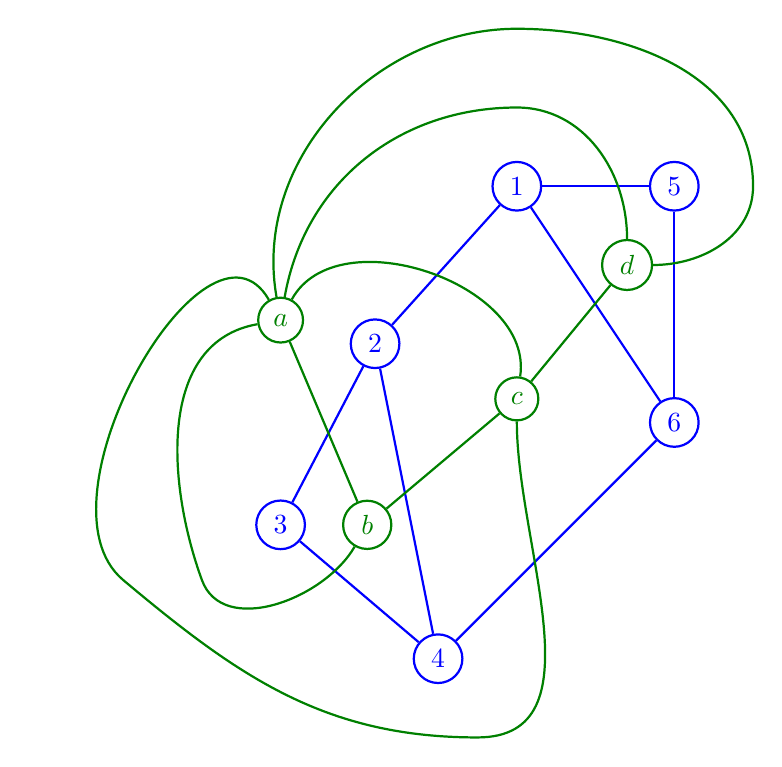
\begin{tikzpicture}[main/.style = {draw, circle, thick, color = Blue}]
		\node[main] (4) at (0,0) {4};
		\node[main] (3) at (-2,1.7) {3};
		\node[main] (6) at (3,3) {6};
		\node[main] (2) at (-0.8,4) {2};
		\node[main] (5) at (3,6) {5};
		\node[main] (1) at (1,6) {1};
		\node[main, color=Green] (b) at (-0.9, 1.7) {$b$};
		\node[main, color=Green] (a) at (-2, 4.3) {$a$};
		\node[main, color=Green] (c) at (1, 3.3) {$c$};
		\node[main, color=Green] (d) at (2.4, 5) {$d$};
		\draw[thick, color=Blue] (4) edge (3);
		\draw[thick, color=Blue] (4) edge (2);
		\draw[thick, color=Blue] (4) edge (6);
		\draw[thick, color=Blue] (5) edge (6);
		\draw[thick, color=Blue] (6) edge (1);
		\draw[thick, color=Blue] (2) edge (1);
		\draw[thick, color=Blue] (1) edge (5);
		\draw[thick, color=Blue] (2) edge (3);
		\draw[thick, color=Green] (b) edge (c);
		\draw[thick, color=Green] (d) edge (c);
		\draw[thick, color=Green] (b) edge (a);
		
		\coordinate (6') at (4,2);
		\coordinate (3') at (-3, 1);
		
		\draw[thick, color=Green] (b) to[out = 240, in = -70] (3') to[out = 110, in = 190] (a);
		\draw[thick, color=Green, bend left = 80] (a) edge (c);
		\draw[thick, color=Green] (c) to[out=270,in=0] (.5,-1) to[out=180,in=-40] (-4,1) to[out=140, in=120] (a); %TODO
		\draw[thick, color=Green] (d) to[out=90,in=0] (1,7) to[out=180,in=80] (a);
		\draw[thick, color=Green] (d) to[out=0,in=270] (4,6) to[out=90,in=0] (1,8) to[out=180, in=100] (a);
	\end{tikzpicture}
	\caption{A \textcolor{Blue}{primal graph $G$} and its \textcolor{Green}{dual $\dual{G}$}.}
\end{figure}

Also duals in Matroids (and also minors) were inspired from graphs. Now we have encountered only planar graphs. But one can ask what about non-planar ones. By Kuratowsku and the fact that graphic matroids are closed under minor operations we get the following proposition.

\begin{prop}
	$\dual{\M}(K_5)$ (and $\dual{\M}(K_{3,3})$) are not graphic.
\end{prop}

\begin{proof}
	By a contradiction: $\exists G : \M(G) = \dual{G}(K_5)$. By that $|E| = 10, \rank(\dual{\M}(K_5)) = 6 = 10 -4$. Also $|V(G)| = 7$ so average degree is $\frac{20}{7} < 3$. Which means that there exists a vertex $v$ s.t. $\deg(v) = 1$ or 2. This leads to at most 2 edges therefore the size of min edge cut is 2 and so is the size of co-circuit of $\dual{\M}(K_5)$ hence the size of circuit in $\M(K_5)$ is 2 which is a contradiction. Similar argument can be made for $K_{3,3}$.
\end{proof}

From these facts if we have a non-planar graph its dual is \textbf{not graphic}. Therefore we get the following diagram.

\begin{figure}[!ht]\centering
	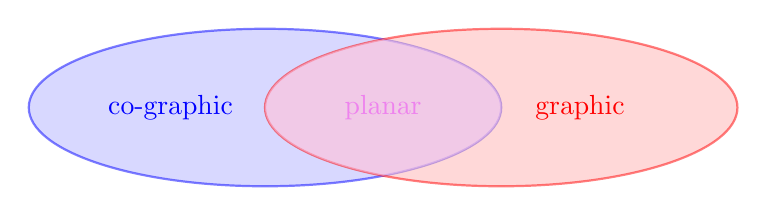
\begin{tikzpicture}[thick]
		\draw[Blue, fill=Blue!30, opacity=.5] (0,0) ellipse (3cm and 1cm);
		\node[Blue] at (-1.2,0) {co-graphic};
		\draw[Red, fill=Red!30, opacity=.5] (3,0) ellipse (3cm and 1cm);
		\node[Red] at (4,0) {graphic};
		\begin{scope}
			\clip (0,0) ellipse (3cm and 1cm);
			\clip (3,0) ellipse (3cm and 1cm);
			\fill[Violet, fill=Violet!40, opacity=.5] (2,0) ellipse (2cm and 1cm);
		\end{scope}
		\node[Violet] at (1.5,0) {planar};
	\end{tikzpicture}
	\caption{Diagram of graphic duals.}
\end{figure}